\lab{Pseudospectra}{Pseudospectra}
\label{lab:pseudospectra}
\objective{Understand and plot the pseudospectra of matrices.}



\section*{Pseudospectra Definition}

The pseudospectrum of a matrix, $\sigma _{\epsilon}(A)$, is a generalization of the point spectrum, or set of eigenvalues, of a matrix. When the entries of a matrix are slightly altered, changes in the point spectrum also occur. The $\epsilon$-pseudospectrum of an $N\times N$ matrix $A$ is defined to be the set of complex numbers, $z$, such that $z$ is in the point spectrum of $A+E$, for some matrix $E$ of the same dimension as $A$ satisfying $\lVert E \rVert < \epsilon$.\\

Note that this definition requires the use of a matrix norm. Any matrix norm can be used, but in this Lab, we will use the norm induced by the 2-norm.\\

One means of plotting the $\epsilon$-pseudospectrum of a $A$ is by generating several random matrices, $E$, with norm $\epsilon$ and plotting the eigenvalues of all of them on the same plot.\\

\begin{figure}
\begin{center}
\begin{subfigure}[b]{.49\textwidth}
\centering
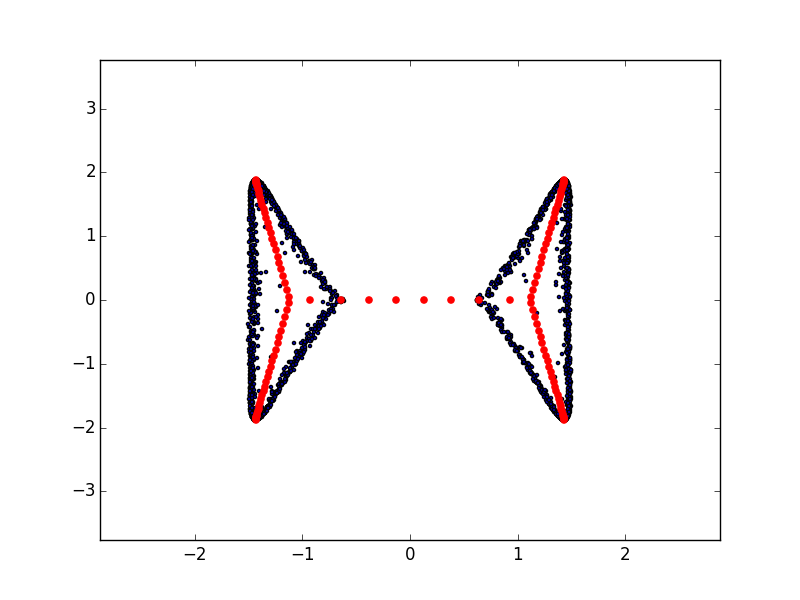
\includegraphics[width=\textwidth]{ps_scatter1}
\end{subfigure}
\begin{subfigure}[b]{.49\textwidth}
\centering
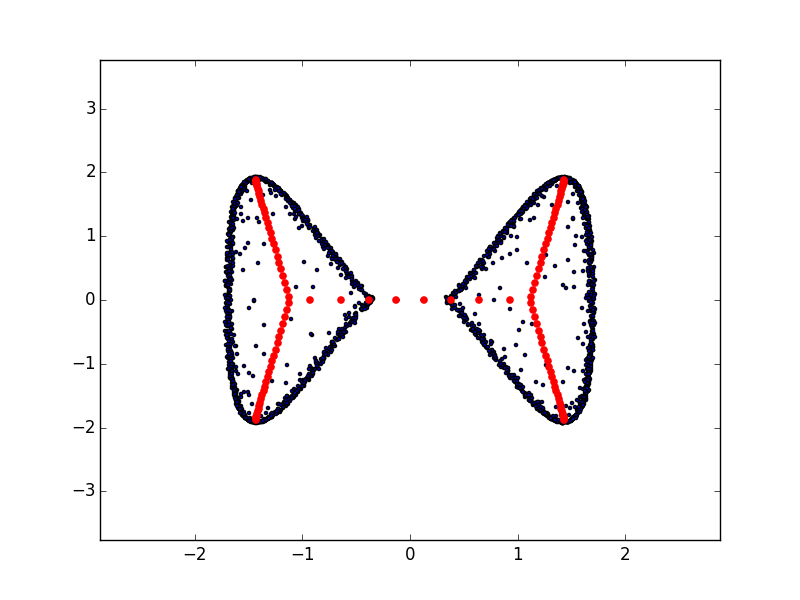
\includegraphics[width=\textwidth]{ps_scatter2}
\end{subfigure}
\caption{Scatter plots representing the $\epsilon$-pseudospectra of the matrix given in Problem 1. The plot on the left uses $\epsilon=10^{-6}$. The plot on the right uses $\epsilon=10^{-3}$. In both plots, the eigenvalues of twenty matrices $A+E$ were plotted.}
\label{fig:ps_scatter}
\end{center}
\end{figure}

\begin{problem}
Complete the function below for plotting the pseudospectrum of a matrix $A$ by plotting the point spectra of several matrices $A+E$, where $\lVert E \rVert = \epsilon$. 

\begin{lstlisting}
def ps_scatter_plot(A, epsilon=.001, num_pts=20):
    '''Plots the 'poorman's pseudospectrum' of a matrix A
    
    Parameters:
    A : square, 2D ndarray
        The matrix whose pseudospectrum is to be plotted
    epsilon : float
        The norm of the random matrices that are generated.
        Defaults to 10**-3
    num_pts : int
        The number of matrices, E, that will be used in the
        algorithm. Defaults to 20.       
    '''
\end{lstlisting}


Have your code also plot the eigenvalues of $A$ in a different color. Test your code on the 120x120 matrix:
\begin{equation}
	\begin{pmatrix}
		0  &  i  &  -1  &  0  & \cdots  &  0  \\
		-i &  0  &   i  & -1 & \ddots  &  \vdots  \\
		1  & -i  &   0  &  i &\ddots&  0  \\
		0   & 1 & -i & 0 &\ddots& -1\\
		\vdots   & \ddots    & \ddots & \ddots &\ddots & i\\
		 0  &  \cdots     &   0     &    1  &   -i  & 0
		\end{pmatrix}
\end{equation}

Your plot should resemble those in Figure \ref{fig:ps_scatter}.
\end{problem}

This method of plotting can only show the $\epsilon$-pseudospectrum of $A$ for one value of $\epsilon$ at a time, and even then it usually just provides a bound for the pseudospectrum. This kind of pseudospectrum plot has been called the poorman's pseudospectrum. In many cases it does not provide sufficient information, so we also plot using a more precise algorithm.

\section*{An Equivalent Pseudospectrum Definition}

One more accurate algorithm depends on a different definition of the $\epsilon$-pseudospectrum of $A$. The pseudospectrum, $\sigma _{\epsilon}(A)$, can also be expressed as 

\begin{equation}
\sigma _{\epsilon}(A) = \{ z \in \mathbb{C} \, | \, \lVert (zI_n-A)^{-1} \rVert > \epsilon ^{-1}\}	
\end{equation}

Note that if $z$ is an eigenvalue of $A$, $(zI_n-A)^{-1}$ does not exist. By convention, we say that its norm is $\infty$.

When we are using the induced 2-norm, we get that $\lVert (zI_n-A)^{-1} \rVert$ is the largest eigenvalue of $(zI_n-A)^{-1}$. This is equal to $1/s_{min}(zI_n-A)$, where $s_{min}(zI_n-A)$ is the smallest eigenvalue of $(zI_n-A)$. Hence, we can write

\begin{equation}
\sigma _{\epsilon}(A) = \{ z \in \mathbb{C} \, | \, s_{min}(A-zI_n) < \epsilon \}	
\end{equation}


\section*{The Lanczos Method}

Using this new definition for $\sigma _{\epsilon}(A)$, we can now plot pseudospectra using Lanczos iterations. Lanczos iterations make use of the Arnoldi method described in Lab \ref{lab:kry_arnoldi} in order to more efficiently compute the smallest eigenvalue of $(zI_n-A)$. This method allows us to plot the pseudospectrum as a contour plot, where each contour corresponds to a fixed value of $\epsilon$. The algorithm is provided below.

\begin{algorithm}
\begin{algorithmic}[1]
\Procedure{Pseudospectrum}{$A, epsilon, xvals, yvals$}
	\State $T \gets schur(A)$			\Comment{Compute the Schur decomposition of A}
	\State $sigmin \gets \zeros{m}{m}$
	\State $Q[:,0] \gets \b/\norm{\b}_2$							
	\For{$k=0\ldots m-1$}
	    \For{$j=0\ldots m-1$}		
		    \State $T_1 \gets (xvals[k]+i*yvals[j])I_N-T$  
		    \State \Comment{$I_N$ is the $N\times N$ identity matrix.}
		    \State $T_2 \gets T1^*$        \Comment{Compute the conjugate transpose.}		
		    \State $sigold \gets 0$    \Comment{Initialize variables.}
		    \State $qold \gets \zeros{N}{1}$
		    \State $beta \gets 0$
		    \State $H \gets \zeros{N}{N}$
		    \State $q \gets$ random, complex-valued $N \times 1$ array of norm 1 
		    \State \Comment{Assume both real and imaginary parts are normally distributed}
		    \For{$p=0 \ldots N-2$}
			    \State $b_1 \gets$ solution to $T_2x = q$	
			    \State $b_2 \gets$ solution to $T_1x = b_1$
			    \State $v \gets b_2 - beta*qold$
			    \State $alpha \gets real(q^**v)$
			    \State $v \gets v - alpha*q$
			    \State $beta \gets \norm{v}$
			    \State $qold \gets q$
			    \State $q \gets v/beta$
			    \State $H[p+1,p] \gets beta$
			    \State $H[p,p+1] \gets beta$
			    \State $H[p,p] \gets alpha$
			    %\State $eigsH \gets$ eigenvalues of $H[:p+1,:p+1]$
			    \State $sig \gets$ absolute value of largest eigenvalue of $H[:p+1,:p+1]$
			    \If{$|sigold/sig-1|<0.001$}
			        \State Break    \Comment{End loop if $sig$ is close to $sigold$}
			    \EndIf
			    \State $sigold \gets sig$
			\EndFor
			\State $sigmin[i,k] \gets \sqrt{sig}$
	    \EndFor
	\EndFor
	\State Plot the log of the values in $sigmin$ as a contour plot on the grid determined by $xvals$ and $yvals$.
\EndProcedure
\end{algorithmic}
\caption{The Lanczos Method. This algorithm accepts a square matrix, $A$; a value or list of values for $\epsilon$; and two one-dimensional arrays of length $m$, $xvals$ and $yvals$. It computes the $10^{-\epsilon}$-pseudospectrum of $A$ for each value of $\epsilon$ and produces the contour plot on the grid determined by $xvals$ and $yvals$.}
\label{alg:lanczos_method}
\end{algorithm}

Note that while this algorithm gives better results than our previous method of plotting pseudospectra, it is much slower.

\begin{figure}
\begin{center}
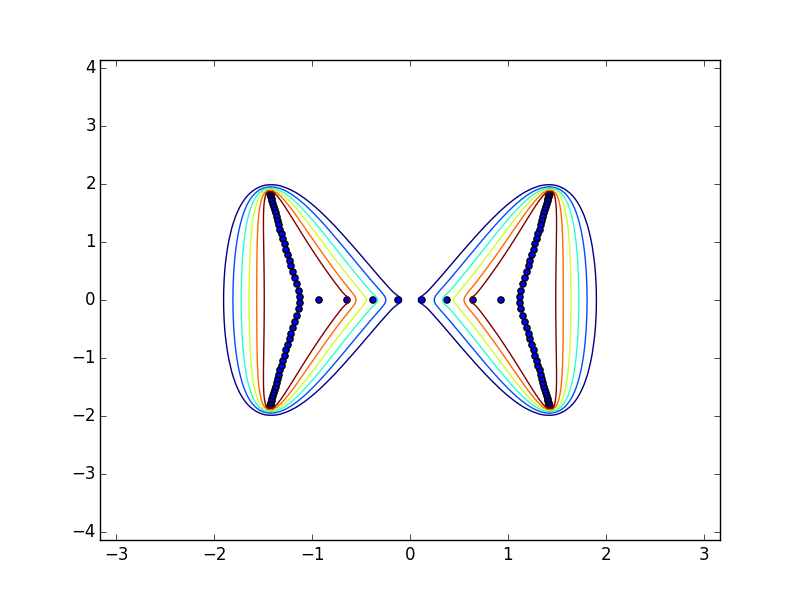
\includegraphics[width=\textwidth]{ps_contour}
\caption{Contour plot of the $\epsilon$-psuedospectrum of the matrix given in Problem 1, with $\epsilon=10^{-2},10^{-3},\cdots,10^{-7}$. }
\label{fig:ps_contour}
\end{center}
\end{figure}



\begin{problem}
Finish the function below for implementing Algorithm \ref{alg:lanczos_method} in Python. Make the function also plot the eigenvalues of the matrix on the same plot.

\begin{lstlisting}
def ps_contour_plot(A, epsilon_vals=None):
    '''Plots the pseudospectrum of the matrix A as a contour plot
    
    Parameters:
        A : square, 2D ndarray
            The matrix whose pseudospectrum is to be plotted
        epsilon_vals : list of floats
            If k is in epsilon_vals, then the epsilon-pseudospectrum
            is plotted for epsilon=10**-k
            If epsilon_vals=None, the defaults of plt.contour() are used
            instead of any specified values.
     '''
    
\end{lstlisting}

Test your code on the matrix from Problem 1. Your plot should look like Figure \ref{fig:ps_contour}. You will need to choose a grid on which to plot the values computed in this algorithm. Use a grid that is roughly twice as large as one needed to plot the eigenvalues. To make your code run faster, make sure to use functions designed for Hermitian or triangular matrices whenever possible.

\end{problem}

\section*{Normal and Nonnormal Matrices}
Recall that a matrix $A$ is normal if it commutes with its conjugate transpose. In the case that $A$ is normal, it can be shown that the $\epsilon$-pseudospectrum consists of the union of circular sets about each of the eigenvalues of $A$. When $A$ is not a normal matrix, the pseudospectrum can have more varied shapes. Because of this, plotting the pseudospectrum of a nonnormal matrix can provide more information about its behavior.

Figure \ref{fig:ps_normal} provides an example of this. The plots show the pseudospectra of the matrices:

\begin{equation}
	B = \begin{pmatrix}
		-1 & 0 & 0\\
		0 & 1 & 0\\
		0 & 0 & i
	\end{pmatrix}, \qquad 	B' = \begin{pmatrix}
		-1 & -1 & -1\\
		0 & 1 & 1\\
		0 & 0 & i
	\end{pmatrix}
\end{equation}

Note that these matrices have the same same set of eigenvalues, and that $B$ is normal, while $B'$ is not. The plot of the pseudospectrum of $B$ shows the expected circular regions, but the plot for $B'$ lacks such symmetry. Another example of this can be seen in Figure \ref{fig:ps_scatter}. The pseudospectrum does not expand out from all of the eigenvalues evenly. Most of the region contained in the pseudospectrum lies on the sides of the plot, and not close to the center.\\

Because the pseudospectra of normal matrices behave so consistently, the study of pseudospectra focuses on nonnormal matrices. Pseudospectra can also be used to study infinite-dimensional linear operators, but different methods are required for plotting their pseudospectra.

\begin{figure}
\begin{center}
\begin{subfigure}[b]{.49\textwidth}
\centering
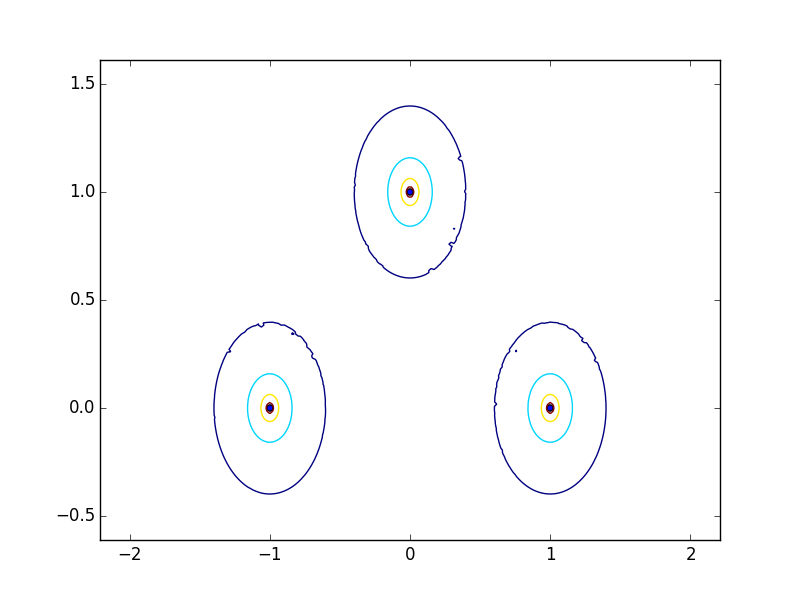
\includegraphics[width=\textwidth]{ps_normal}
\end{subfigure}
\begin{subfigure}[b]{.49\textwidth}
\centering
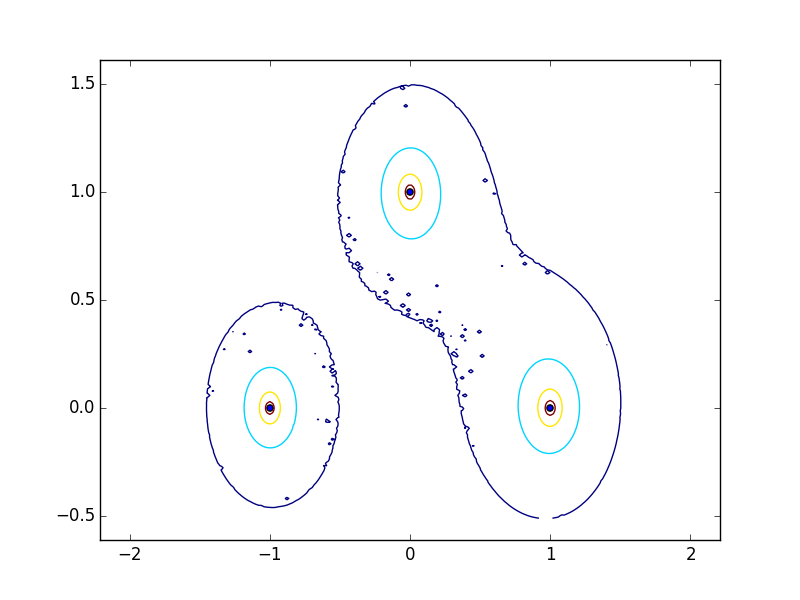
\includegraphics[width=\textwidth]{ps_nonnormal}
\end{subfigure}
\caption{Plots of the Pseudospectrum of two matrices with the same eigenvalues. The plot on the left is for a normal matrix, and the one on the right is for a nonnormal matrix. The contours correspond to $\epsilon=10^{-0.4},10^{-0.8},10^{-1.2}$}
\label{fig:ps_normal}
\end{center}
\end{figure}

~\cite{Tufte2005}



